\section{昂贵黑箱问题}
\label{sec:bo-problem}

只有$T$次昂贵评价时，优化问题应当怎样提？设搜索域$\bm{C}\subseteq\mathbb{R}^n$已知，目标$f:\bm{C}\to\mathbb{R}$的表达式未知，要解的是
\begin{equation}
 \min_{\bm{x}\in\bm{C}}\ f(\bm{x}),
 \label{eq:bo-problem}
\end{equation}
其中每次只能选一个$\bm{x}$，付出一次运行的代价，读到一个函数值。这类只能通过读数了解目标的问题称为\term{黑箱优化}（black-box optimization）。

与前面各章不同，这里最先固定的不是精度，而是预算：允许多少次评价，或者总共多少运行时间。问题随之变成“这$T$次机会怎样分配”。机会要分给两类地方：看起来有希望的区域，以及几乎一无所知的区域。只去前者可能错过别处更深的谷，只去后者又用不上已经学到的东西。

\paragraph{贯穿全章的例子}
设仿真参数$x$在$\bm{C}=[0,8]$内取值，输出误差$f(x)$已作标准化，负值表示比基准好，预算$T=6$。表~\ref{tab:bo-readings}列出整数位置上的读数。真实计算时这张表并不存在，算法只会知道被评价过的那几列；把它写出来是为了让后面的每一步都可以核对。

\begin{BookInlineTable}
 \centering
 \caption{贯穿例的整数位置读数。函数$f$是过这九个点的自然三次样条，只作为教学假设，算法不知道它。}
 \label{tab:bo-readings}
 \begin{tabular}{cccccccccc}
 \toprule
 $x$&0&1&2&3&4&5&6&7&8\\
 \midrule
 $f(x)$&0.9&0.2&$-0.5$&0.1&0.7&0.3&$-1.0$&$-0.3$&0.8\\
 \bottomrule
 \end{tabular}
\end{BookInlineTable}

这个函数有两个谷，一个在$x=2$附近，另一个在$x=6$附近，后者更深。样条的最小值约为$-1.029$，在$x\approx6.13$处取得。

\subsection{评价点与推荐解}
\label{sec:bo-query-recommend}

六次评价结束后要交出一个答案。答案未必是读数最好的那次，也未必是评价过的点。为了不把两件事混在一起，需要分开两个角色：\emph{评价点}用来收集信息，\emph{推荐解}用来实际采用。

图~\ref{fig:bo-query-recommend}是后面算法在贯穿例上实际走出的六次评价，数字是评价的先后。第$4$次去了$x=8$，读数$0.8$很差，从目标值看是一次失败。可是它告诉我们右端不值得再投入，这对后面的判断有用。第$5$次在$x=6$读到$-1.0$，于是最终推荐$\widehat{x}_6=6$。第$6$次在$x=0$的读数$0.9$又差得多，但这并不影响推荐，因为推荐解不需要是最后一次评价。

\begin{BookInlineFigure}
 \centering
 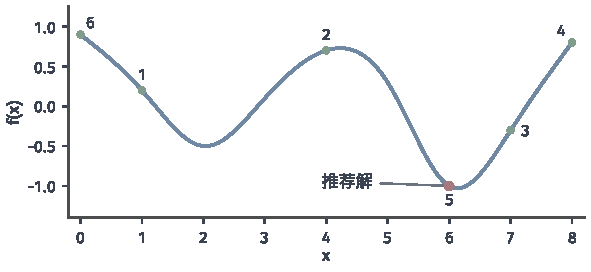
\includegraphics[width=100mm]{figures/05-optimization/05-stochastic-optimization/matplotlib/bo-query-recommend/figure.pdf}
 \caption{评价点与推荐解。蓝线是目标$f$，绿点是六次评价，旁边的数字是评价顺序，红点是最终推荐。第$4$次和第$6$次的读数很差，它们的任务是收集信息，不是交付答案。}
 \label{fig:bo-query-recommend}
\end{BookInlineFigure}

用数据集合记录当前已有的信息。设前$t$次评价的位置与读数为$(\bm{x}_i,y_i)$，记
\begin{equation}
 \mathcal{D}_t=\{(\bm{x}_i,y_i)\}_{i=1}^t.
 \label{eq:bo-data}
\end{equation}
这里下标$i$表示第$i$次评价，因为后面总要同时引用多次评价的位置，所以本章把评价序号写在下标。

选点规则必须遵守时间次序：第$t+1$个评价点只能依赖$\mathcal{D}_t$，至多再加上与目标无关的随机数，不能用尚未返回的读数。图~\ref{fig:bo-info-timeline}画出了这个次序。这条要求看似多余，实际很有约束力。比较不同方法时，若某个方法的超参数是用全部读数调好的，它在前几步就已用到了未来的信息，比较便不公平。

\begin{BookInlineFigure}
 \centering
 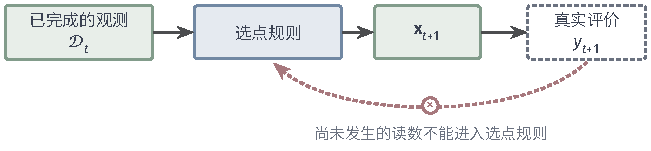
\includegraphics[width=110mm]{figures/05-optimization/05-stochastic-optimization/tikz/bo-info-timeline/figure.pdf}
 \caption{选点规则可以使用的信息。选点规则只读取已完成的观测$\mathcal{D}_t$，下一次评价的读数$y_{t+1}$在选点之后才产生（虚线框），红色虚线表示这条信息通路不允许存在。}
 \label{fig:bo-info-timeline}
\end{BookInlineFigure}

\subsection{概率模型的作用}
\label{sec:bo-probability-role}

只有三个读数时，$x=6$处的函数值是多少？我们不知道，但并非毫无看法：离读数近的地方函数值大概与读数接近，离得远的地方拿不准。要把“大概”和“拿不准”写成可以计算的东西，需要给未知的$f$配一个概率描述。

这里最容易误解的一点是，$f$本身并不随机。仿真程序是确定的，同一个$x$每次算出同样的结果，只是我们不知道结果。概率描述的是我们的认识状态，不是目标的物理性质。做法是引入一个随机函数$F$作为模型，把$f$看成它可能的一种情形。在看到数据之前，$F$的分布称为\term{先验}（prior）；把$\mathcal{D}_t$作为条件之后，$F$的分布称为\term{后验}（posterior）。

后验分布的变化，表示认识变了，不表示目标变了。可以把它想成一张还在绘制中的地形图：实地地形一直没动，测过的点清晰，没测过的地方模糊，每多测一点，图就清楚一些。这个比方有一处不准确：地形图的模糊只来自没测量，而概率模型的结论还依赖我们事先对地形光滑程度的假设，假设错了，图可能清晰却画错了。

图~\ref{fig:bo-consistent-functions}中的紫线是在$x=1,4,7$三个读数条件下，从模型里抽取的几条函数。它们都穿过三个读数，在读数之间各走各的路。蓝线是真实目标，只有一条，它在整个过程中不改变。浅蓝带是模型认为函数值大致所在的范围，读数处收成一点，远离读数时变宽。下一次评价的放置，就要根据这种“哪里可能低、哪里还拿不准”的信息来定。

\begin{BookInlineFigure}
 \centering
 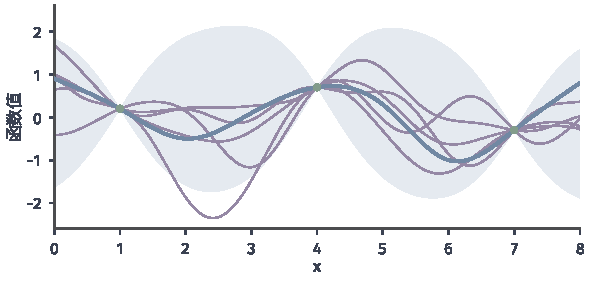
\includegraphics[width=100mm]{figures/05-optimization/05-stochastic-optimization/matplotlib/bo-consistent-functions/figure.pdf}
 \caption{固定的目标与模型的多种可能。粗蓝线是真实目标$f$，绿点是$x=1,4,7$的读数，细紫线是后验分布的五个样本，浅蓝带是后验均值上下各两倍标准差。五条紫线都与读数相符，它们的差异表示认识的不确定，不表示$f$在变化。}
 \label{fig:bo-consistent-functions}
\end{BookInlineFigure}

概率模型是本章区别于前两章的关键。三章都可以只用函数值，分工却在于用这些值做什么，表~\ref{tab:bo-three-methods}作了对比。也要注意，“贝叶斯”这个词不意味着算法每步都在抽签。后面的期望改进给定$\mathcal{D}_t$后完全确定，只有Thompson采样这样的规则才主动使用随机数。

\begin{BookInlineTable}
 \centering
 \caption{三种只用函数值的做法。}
 \label{tab:bo-three-methods}
 \begin{tabular}{lll}
 \toprule
 &用读数做什么&适合的评价预算\\
 \midrule
 零阶随机优化&差分成局部方向&较多，随维数增长\\
 随机搜索&更新搜索状态或分布&较多，候选大量淘汰\\
 贝叶斯优化&建模后计算下次评价的价值&很少，每次都很贵\\
 \bottomrule
 \end{tabular}
\end{BookInlineTable}
